%
% Chapter 8
%

\chapter{BACKGROUND PREDICTIONS}
Despite optimizing the event selection criteria to select signal events, a substantial amount of background events from a variety of processes enter the signal region.
These backrounds are classified as being either reducible or irreducible inside the signal region, and are estimated differently depending on the classification. An understanding
of each background process and a proper assessment of the uncertainity associated with the estimation of each background is critical to extracting the signal and interpreting
the results. 

\section{Reducible backgrounds}
Reducible backgrounds arise from a number of sources, but always contain leptons that are either non-prompt, or have a lepton whose electric charge is mismeasured.
Reducible backgrounds are estimated from data-driven approaches using control regions and extrapolation techniques to predict their contribution to the signal region yield. 
They are called reducible because, if the signal region and CMS event reconstruction worked with perfect efficiency they would not enter the signal region, thus working
to improve prompt lepton identifiction and CMS lepton electric charge measurement can reduce the contributions from these processes. The background due to fakes is entirely
separate from the charge mismeasurement background and are estimated separately. 

\subsection{Fake lepton background}    
The background due to fake or non-prompt leptons is primarily due to the relatively large-cross-section semi-leptonic \ttbar process, where the b-jet from the leptonic top quark
produces a fake (non-prompt) lepton that passes the tight lepton selection criteria, but also includes other processes where a lepton is produced inside a jet. The background from
these events is estimated via a loose-to-tight extrapolation. This begins with measuring the rate at which leptons passing the fakeable selection also pass the tight selection in a
control region with data. This measurement is then used to extrapolate from a sideband with fakeable leptons to the signal region with
tight leptons to estimate the signal region contribution from to events with fake leptons. 

A control region heavily enriched in QCD multijet events is designed to measure the probability of a non-prompt lepton passing the fakeable selection to also pass the tight selection.
This probability is called the fake rate, and the control region is referred to as the measurement region. The measurement region requires events with one loose lepton and one
hadronic jet isolated from the lepton with $\Deta$R $\gt$ 0.7. This definition enriches the measurement region with non-prompt leptons. The data analyzed in the measurement region is collected on single lepton
triggers which require a lepton with \pt $\gt$ 30 GeV, and a particle-flow jet with \pt $\gt$ 30 GeV.

Additional requirements to ensure closure with \ttbar MC  

\subsection{Charge mismeasurment background}

\section{Irreducible backgrounds}
Irreducible backgrounds are estimated strictly from MC. Irreducible backgrounds earn their name from the fact that even if the signal region and CMS event/object reconstruction
worked with perfect efficiency, they still contain the necessary objects to consistently pass the signal region selection and are thus irreducible with resepect to the signal
region definition. The dominant irreducible background processes include \ttw and \ttz. Other irreducible background processes include diboson pairs produced in association with jets,
while smaller contributions include processes with a single W or Z boson, a single top quark, tribosons, as well as other rare\footnote{Rare means a very small cross section, and very
small background contribution} SM backrounds. The modelling of these background processes has been checked to ensure a good agreement among the variable used to event selection and
signal extraction.  


%% \begin{figure}[hbtp]
%%  \begin{center}
%%    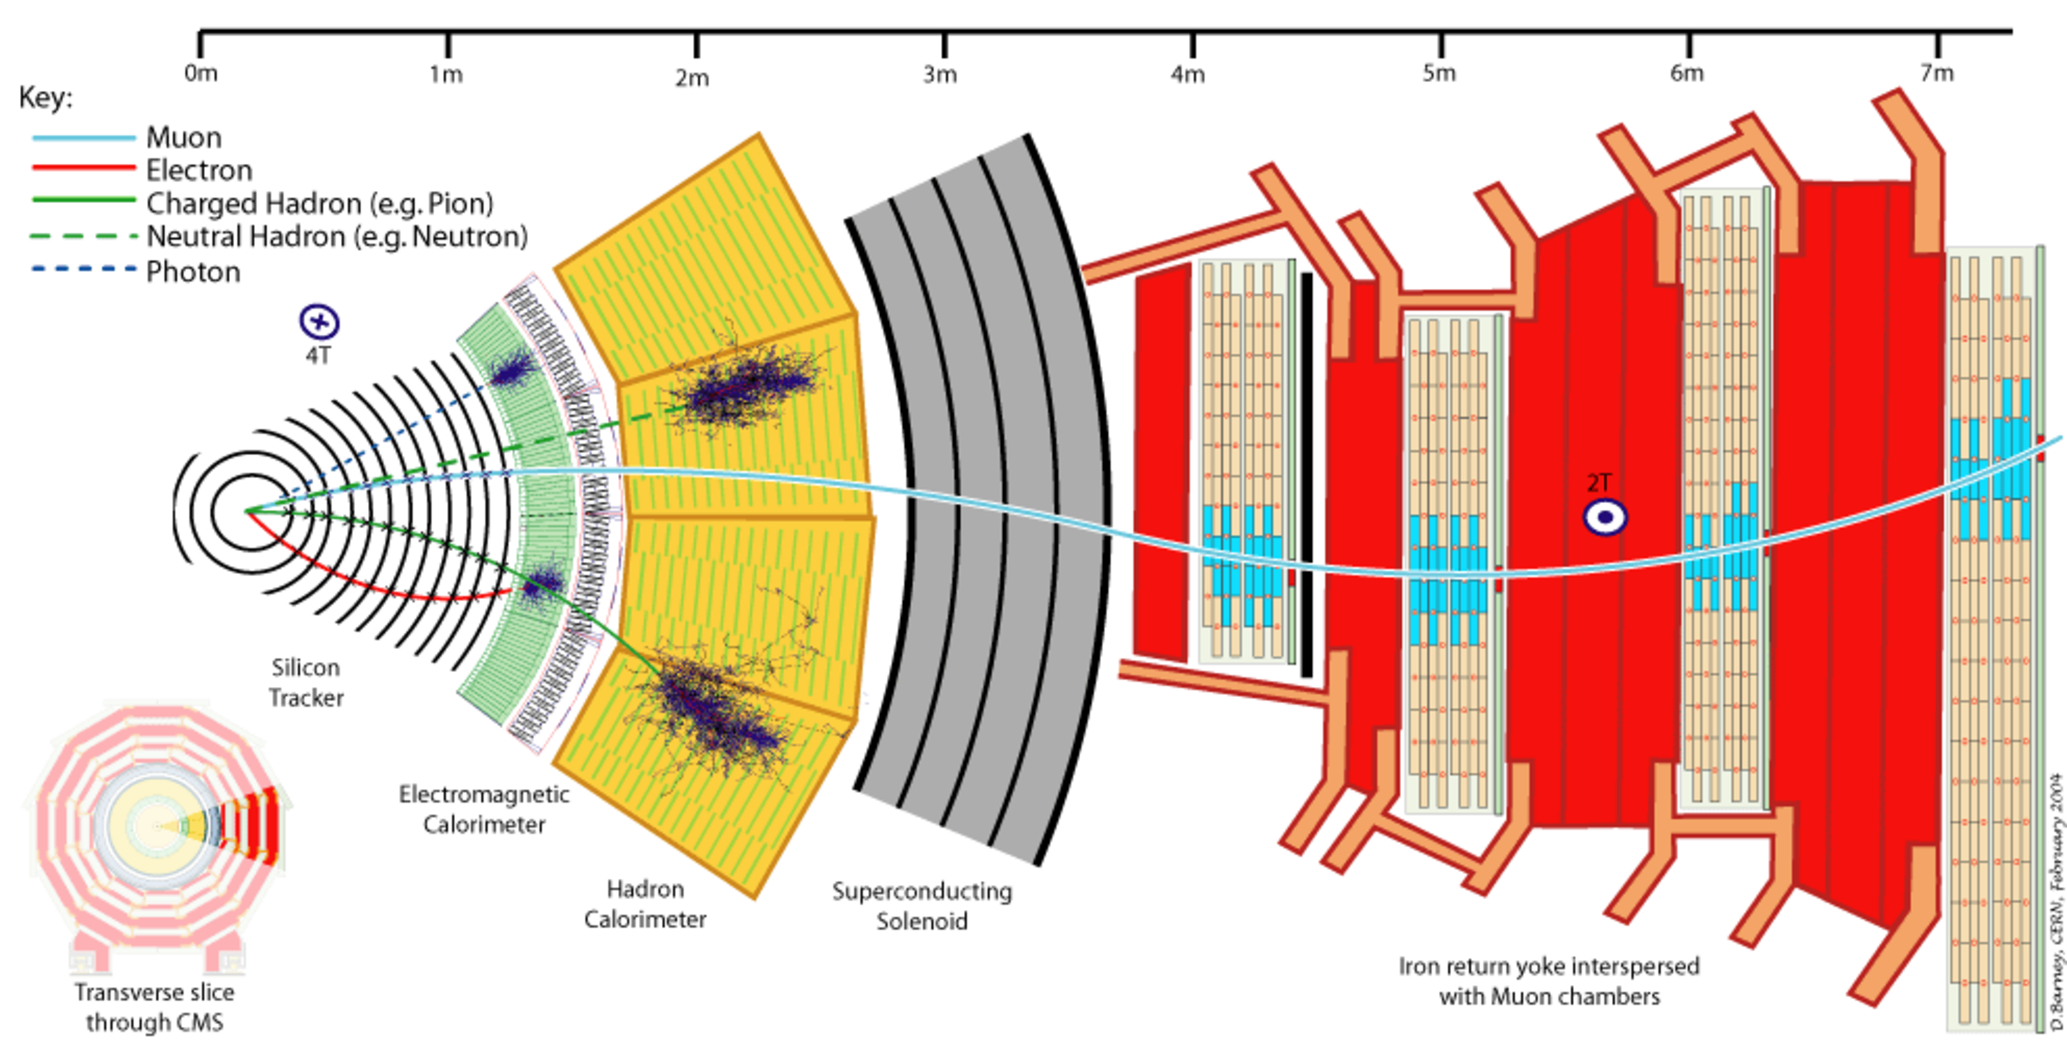
\includegraphics[width=0.8\textwidth]{ch4_figs/cms_particleflow.pdf}
%%    \caption{An overview of how CMS detects different types of particles. The slice of CMS in in the x-y plane.~\cite{NEED CITATION}.}
%%    \label{fig:cms_pflow}
%%  \end{center}
%% \end{figure}
